\def \ratiovolwidth {0.5}
\def \ratiovolheight {0.4}
\def \ratiovolhorshift {0cm}
\def \ratiovolvertshift {-2cm}

\begin{figure}
  \vspace*{\ratiovolvertshift}
  \hspace*{\ratiovolhorshift}\subfloat[5 Lin]{
  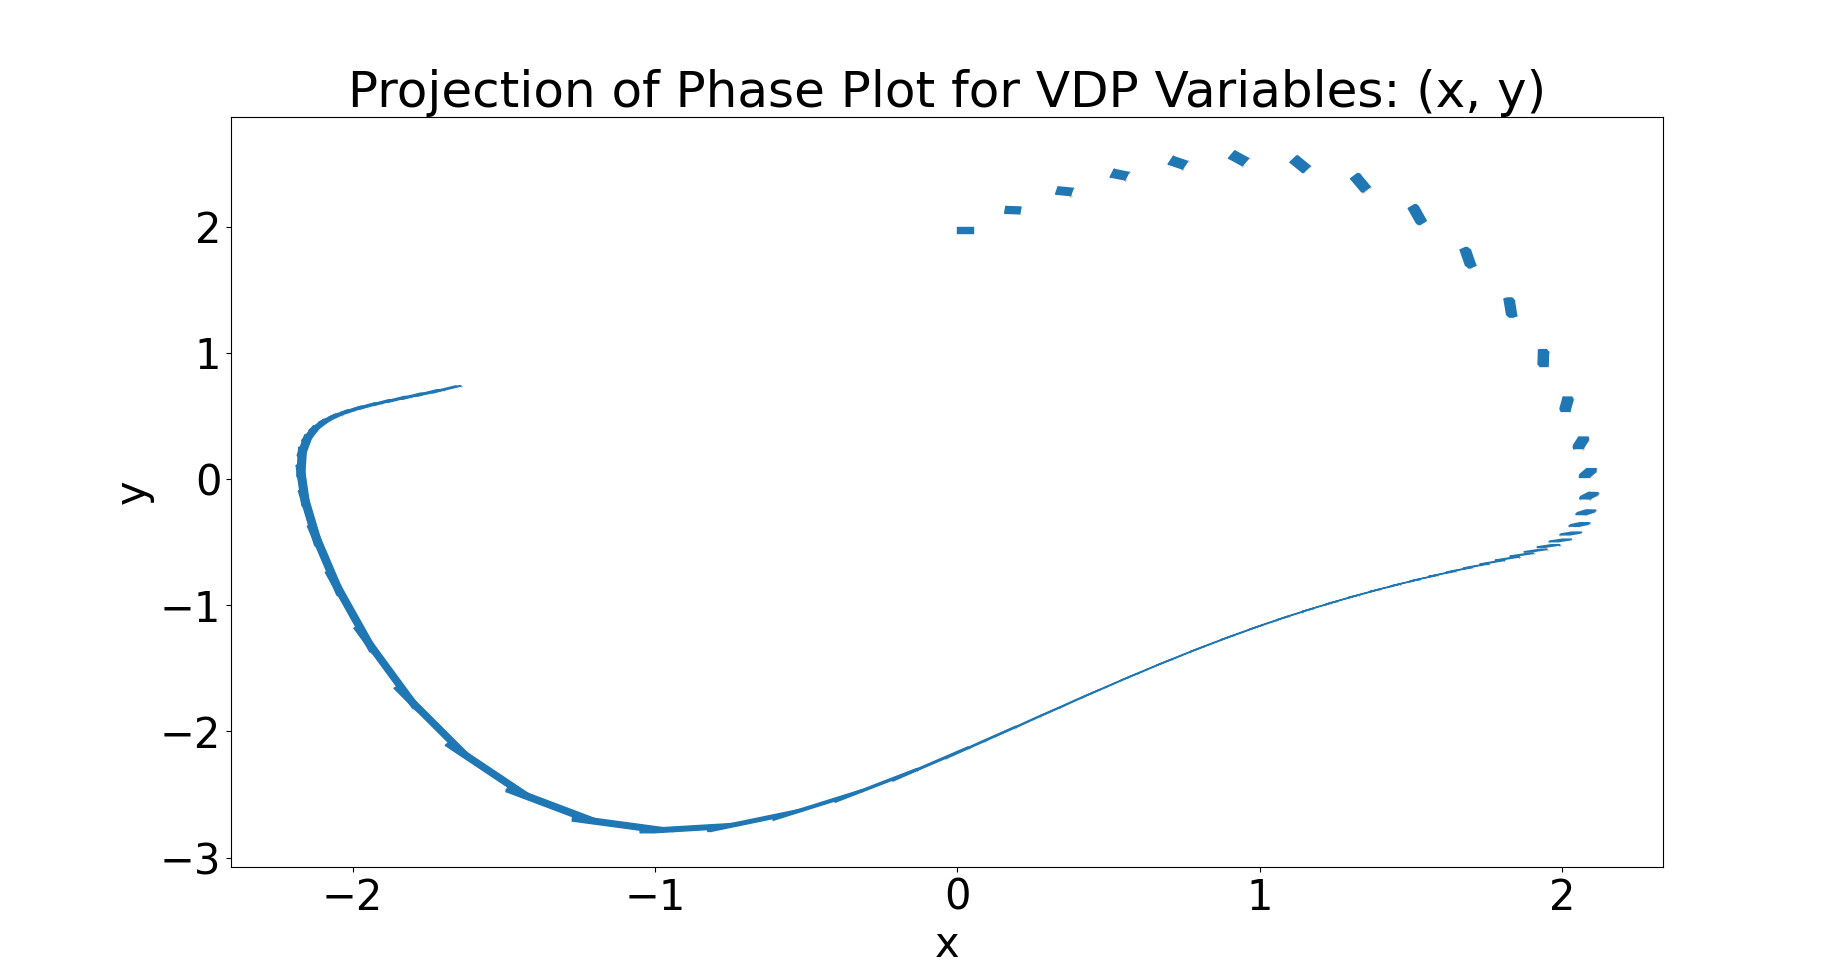
\includegraphics[width=\ratiovolwidth\textwidth, height=\ratiovolheight \textwidth]{figures/PhasePlots/VDP_5Lin_.png}
}
\subfloat[1 PCA 5 Lin]{
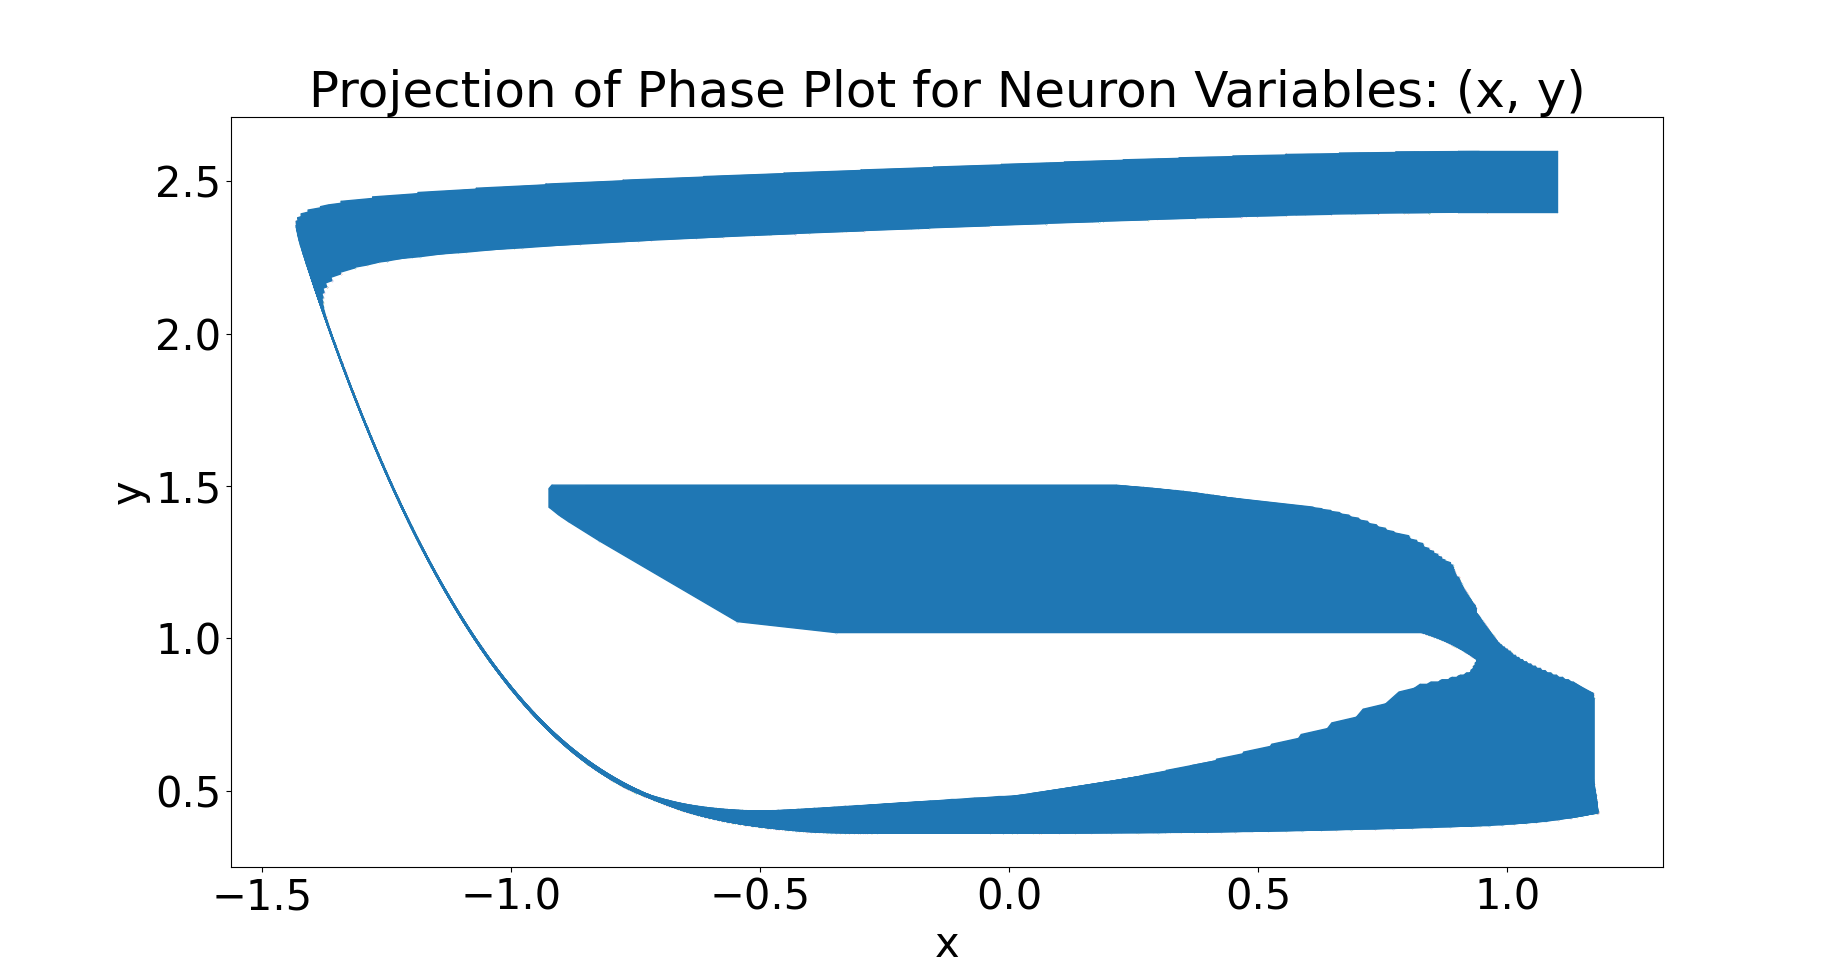
\includegraphics[width=\ratiovolwidth\textwidth, height=\ratiovolheight \textwidth]{figures/PhasePlots/Neuron_1PCA5Lin_.png}
}

\hspace*{\ratiovolhorshift}\subfloat[5 PCA]{
  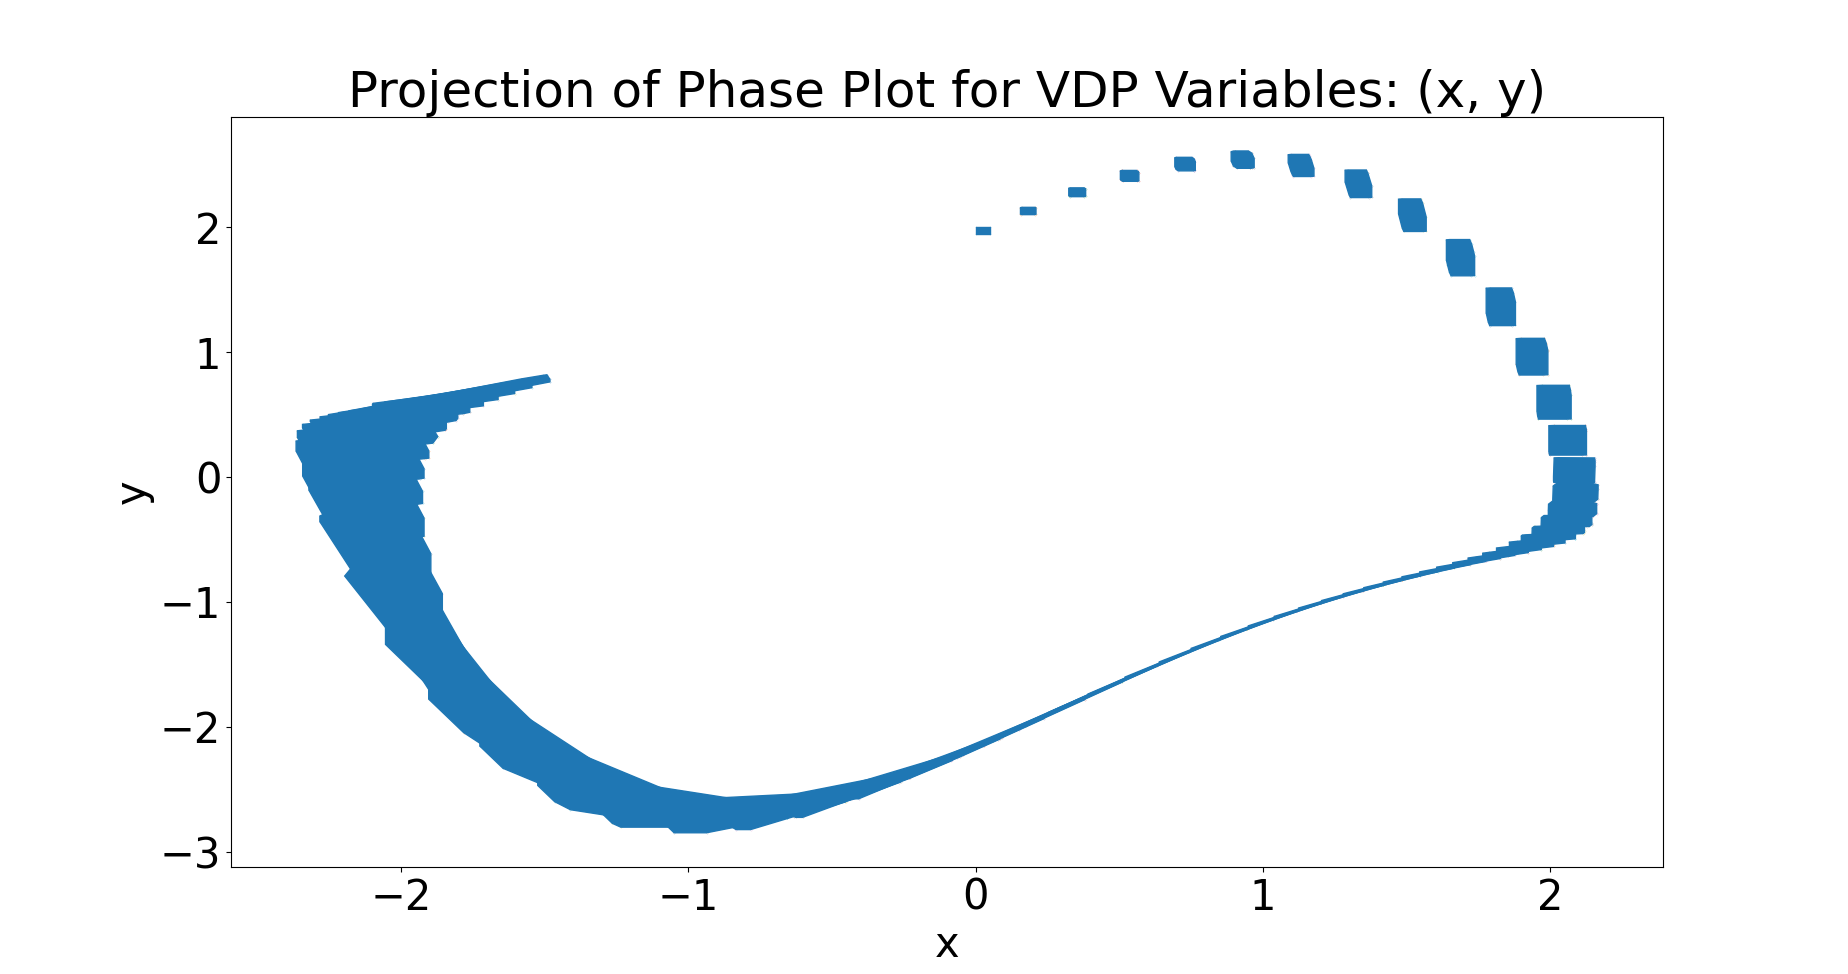
\includegraphics[width=\ratiovolwidth\textwidth, height=\ratiovolheight \textwidth]{figures/PhasePlots/VDP_5PCA_.png}
}
\subfloat[5 PCA 1 Lin]{
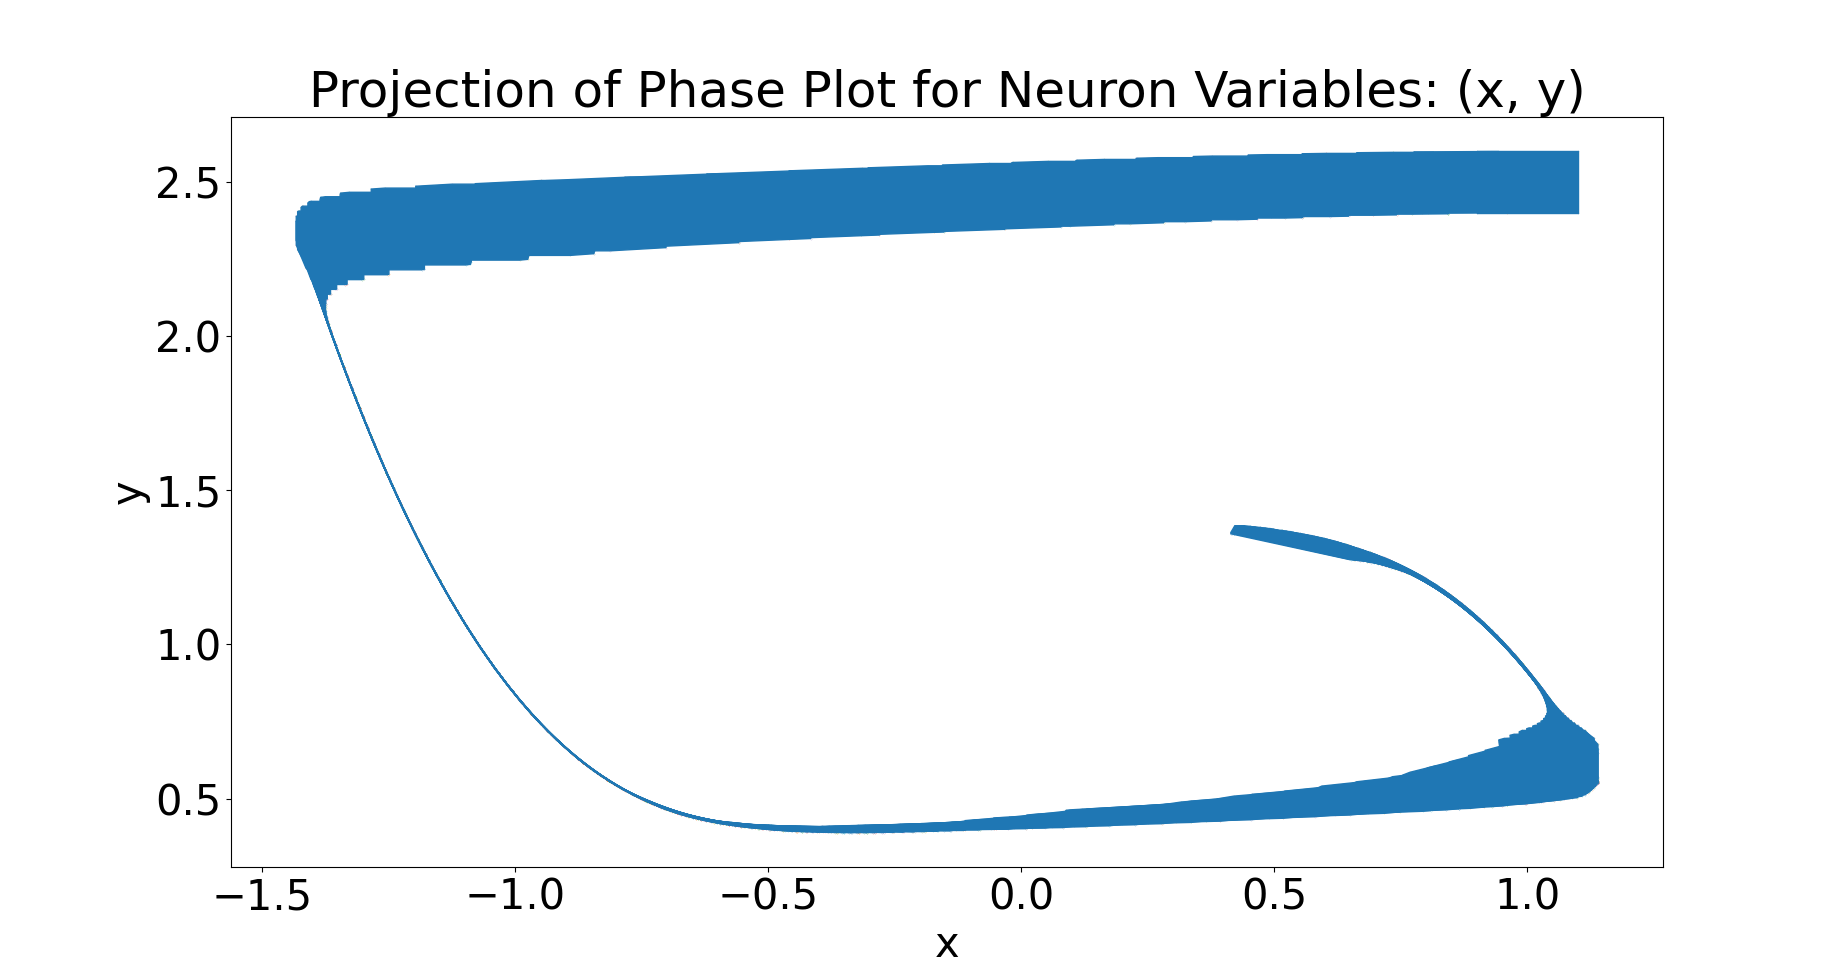
\includegraphics[width=\ratiovolwidth\textwidth, height=\ratiovolheight \textwidth]{figures/PhasePlots/Neuron_5PCA1Lin_.png}
}

\hspace*{\ratiovolhorshift}\subfloat[Sapo]{
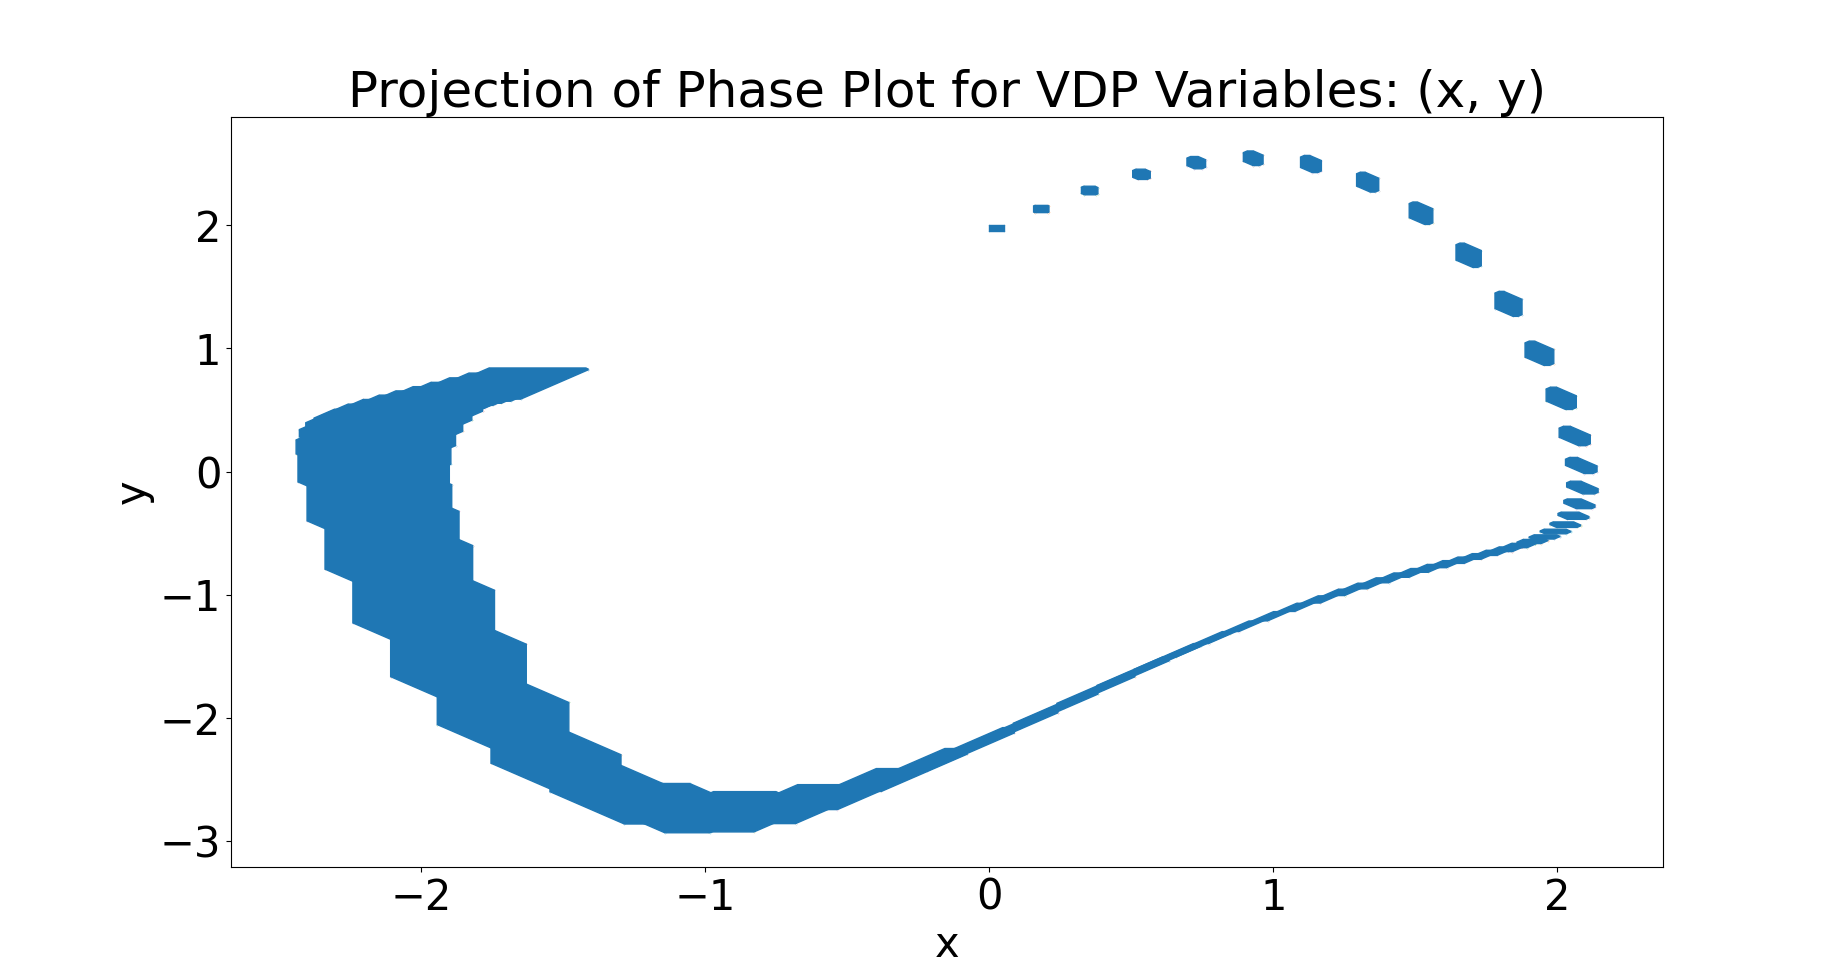
\includegraphics[width=\ratiovolwidth\textwidth, height=\ratiovolheight \textwidth]{figures/PhasePlots/VDP_Sapo_.png}}
\subfloat[Sapo]{
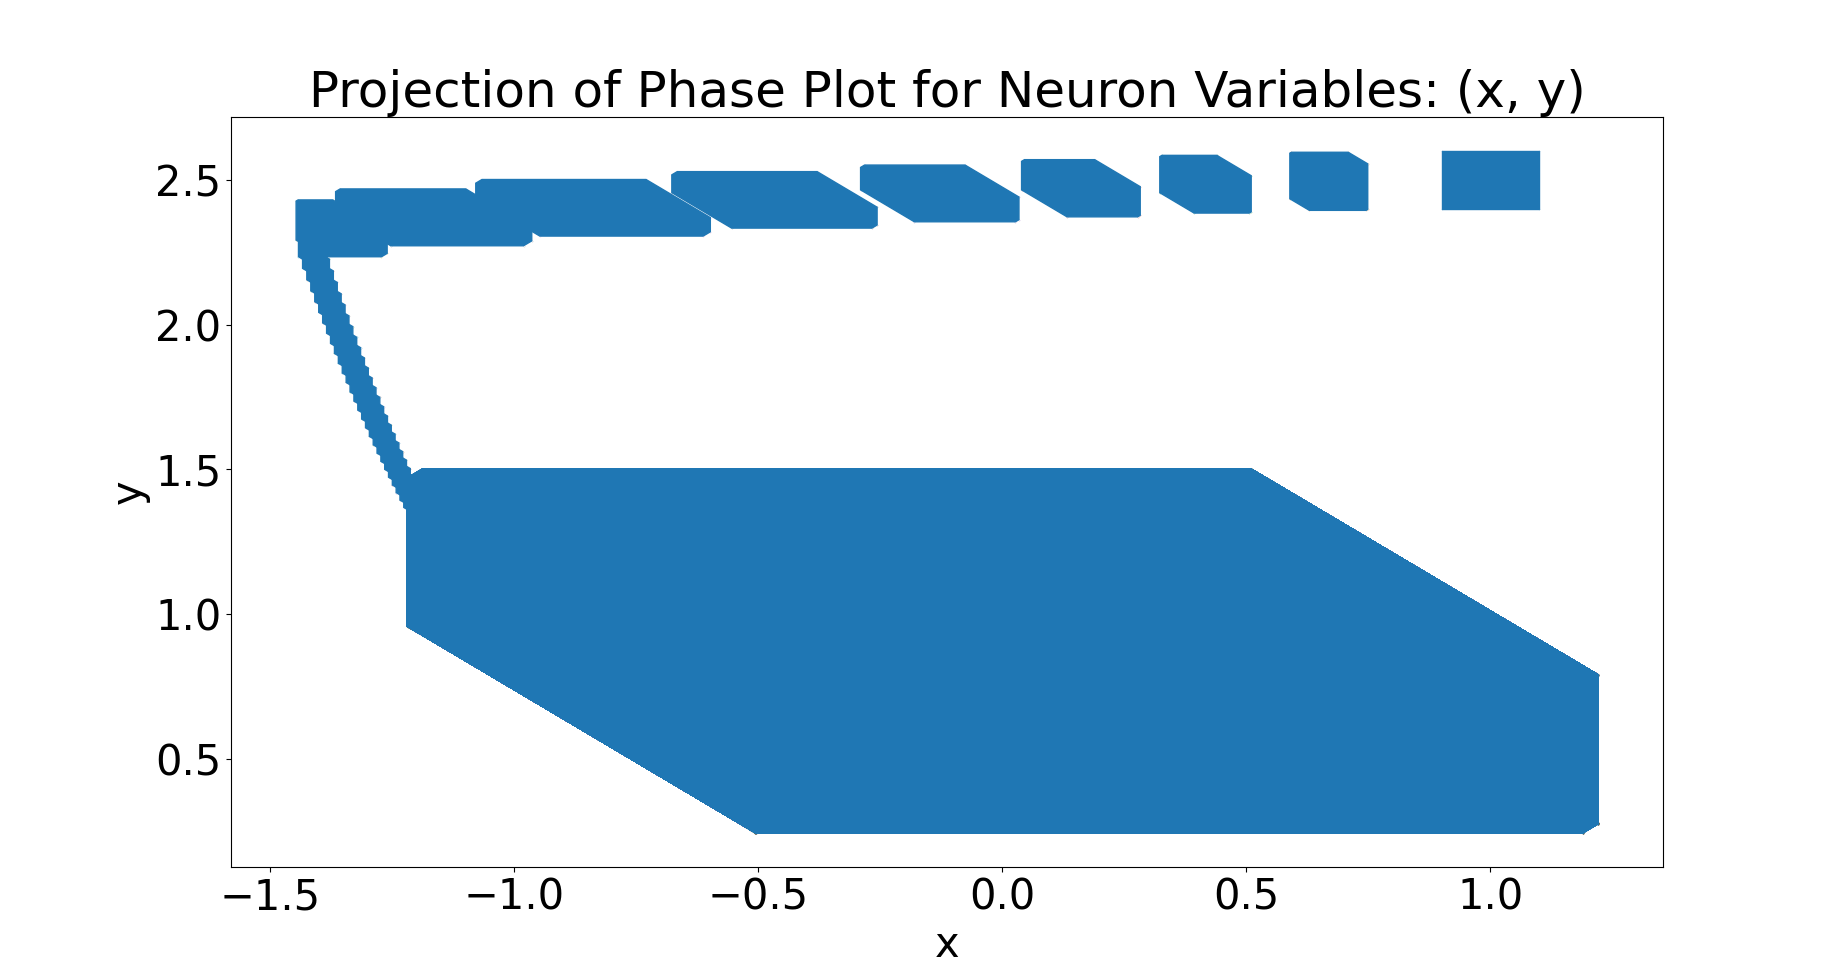
\includegraphics[width=\ratiovolwidth\textwidth, height=\ratiovolheight \textwidth]{figures/PhasePlots/Neuron_Sapo_.png}
}

\caption{Effect of varying ratio between the number of PCA and Linear Approximation parallelotopes. The Vanderpol (left) and the FitzHugh-Nagumo Neuron (right) phase plots are shown to illustrate differing effects of varying the PCA/LinApp ratio. The initial set for the Vanderpol model is set to $x \in [0,0.05], \, y \in [1.95,2]$, and the initial set Neuron model is set to $x \in [0.9, 1.1], \, y \in [2.4,2.6]$}
\label{fig:PCALinAppRatio}
\end{figure}
